\chapter{Access Control}
\label{ch:access_control}

\section{Introduction to Access Control}
Access control is fundamentally a binary decision mechanism: whenever an entity requests access to a resource, the system must determine whether the action is \textit{allowed} or \textit{denied}. While this concept appears simple on the surface, scaling this binary decision across thousands of users and millions of resources in a modern computing environment is profoundly complex. Administrators cannot explicitly list the answers for every possible access request; instead, they must distill these permissions into robust and generalized \textit{rules}.

The study of access control revolves around three primary questions:
\begin{enumerate}
    \item How do we \textit{design} the access rules?
    \item How do we \textit{express} the access rules in practice?
    \item How do we appropriately \textit{apply} them?
\end{enumerate}

\subsection{Authentication and Authorization}
Before access control can take place, the system must establish identities and evaluate policies. This process is split into two phases:
\begin{itemize}
    \item \textbf{Identification and Authentication:} Verifies the identity of the \textit{principal} (the active entity, such as a human user) making the request, mapping them to a corresponding system \textit{subject} (such as a running process).
    \item \textbf{Authorization:} The process where the system evaluates the subject's request to perform an \textit{access operation} on a passive \textit{object} (such as a file or a network socket), checking against established access control policies.
\end{itemize}

While centralized systems handle this cleanly, distributed systems introduce severe complexities regarding how to discover all relevant policies across nodes, and how to safely make decisions when policies may be missing or unreachable.

\section{The Reference Monitor}
The core component responsible for enforcing access control policies within an operating system is known as the \textbf{Reference Monitor}. It is an abstract machine that mediates all access to objects by subjects, answering the question: ``Who does what on which resource?'' All modern operating system kernels implement some form of a reference monitor.

According to the foundational Anderson report (1972), a Reference Monitor must satisfy three stringent requirements:
\begin{enumerate}
    \item \textbf{Tamper-proof:} It must be impossible for malicious subjects to modify or disable the reference monitor's code or its access control policies.
    \item \textbf{Non-bypassable:} Every single request for resource access must pass through the reference monitor. There can be no alternative paths to the resource.
    \item \textbf{Small enough to be verified:} The implementation must be sufficiently compact and simple so that it can be rigorously tested and mathematically or empirically verified to be correct.
\end{enumerate}

\begin{figure}[htpb]
    \centering
    \begin{tikzpicture}[node distance=2.5cm, auto, thick, >=stealth]
        \node[draw, rectangle, fill=blue!10, minimum height=1cm] (principal) {User Identity};
        \node[draw, ellipse, fill=blue!20, right of=principal, node distance=3cm] (subject) {Process};
        \node[draw, rectangle, fill=blue!10, right of=subject, node distance=3.5cm, minimum height=1cm, align=center] (monitor) {Reference\\Monitor};
        \node[draw, rectangle, fill=blue!10, right of=monitor, node distance=3cm, minimum height=1cm, align=center] (object) {File/\\Resource};
        \node[draw, rectangle, dashed, above of=monitor, node distance=2cm, align=center] (policy) {Access Control\\Policies};
        
        \draw[->] (principal) -- node[above] {Auth} (subject);
        \draw[->] (subject) -- node[above] {Request} (monitor);
        \draw[<->] (monitor) -- node[above] {Access} (object);
        \draw[->, dashed] (policy) -- (monitor);
    \end{tikzpicture}
    \caption{The relationship between Principals, Subjects, the Reference Monitor, and Objects.}
    \label{fig:ref_monitor}
\end{figure}

\section{Access Control Models}
Access control models provide the formal framework for how privileges are assigned and evaluated. They can be broadly categorized into three types based on \textit{who} assigns the privileges and how they are structured:
\begin{itemize}
    \item \textbf{Discretionary Access Control (DAC):} The resource owner discretionarily decides who can access their resources.
    \item \textbf{Mandatory Access Control (MAC):} Privileges are strictly set by a central security administrator according to system-wide policies; users cannot override these.
    \item \textbf{Role-Based Access Control (RBAC):} Access is granted based on abstract organizational \textit{roles} rather than raw individual identities.
\end{itemize}
The fundamental difference between DAC and MAC lies precisely in who holds the authority to grant or revoke privileges.

\section{Discretionary Access Control (DAC)}
In a DAC system, the creator or owner of a resource acts as the ultimate authority over it. For example, if Stefano creates a file, he can discretionarily grant Federico the privilege to read it. 

Because this reflects intuitive human ownership, virtually all off-the-shelf operating systems (Windows, Linux, macOS) and applications (like social networks) implement DAC as their primary mechanism.

\subsection{The General Model of DAC (HRU Model)}
To rigorously analyze DAC, we rely on formal models such as the Harrison-Ruzzo-Ullman (HRU) model (derived from Lampson's access matrix). The model identifies three main entities:
\begin{itemize}
    \item \textbf{Subjects ($S$):} Active entities capable of exercising privileges.
    \item \textbf{Objects ($O$):} Passive resources upon which privileges are exercised.
    \item \textbf{Actions ($A$):} Operations that can be performed (e.g., read, write, execute).
\end{itemize}

The \textbf{Protection State} of the system is represented as a triple $(S, O, A)$. The privileges are recorded in an \textbf{Access Control Matrix} $\mathcal{A}$, where $\mathcal{A}[s,o]$ contains the subset of actions $A$ that subject $s$ is authorized to execute on object $o$. 

\subsection{Transitions and Safety Problems}
A system's protection state does not remain static; it undergoes \textit{transitions} via sequences of basic operations. Basic operations include creating or destroying subjects and objects, and adding or removing permissions from the matrix $\mathcal{A}[s,o]$. 

However, transitions must be carefully controlled. A command like ``create file $f$ for user $u$'' must include conditional statements (e.g., checking if $f$ already exists) to prevent hostile takeovers of existing objects.

This dynamicity introduces the \textbf{Safety Problem}: Given an initial configuration and a defined set of transitions, is there any sequence of commands that allows a subject $s$ to obtain a specific right $r$ on an object $f$ without the owner explicitly intending to grant it? If such an unintended leak is possible, the system's commands are \textit{unsafe by design}.

Formally, Harrison, Ruzzo, and Ullman proved that in a generic HRU model with infinite resources, the safety problem is \textbf{undecidable}. It is only mathematically decidable in highly constrained, practically useless environments (such as mono-operational systems) or strictly finite resource bounds.

\subsection{Common Implementations of DAC}
A pure access control matrix is inherently sparse, making it highly inefficient to store directly in memory. Operating systems use alternative data structures:
\begin{itemize}
    \item \textbf{Authorizations Table:} A database table recording only non-null $(S, O, A)$ triples. Commonly used in relational Database Management Systems (DBMS).
    \item \textbf{Access Control Lists (ACLs):} Represents the matrix by \textit{columns}. Each object holds a list of subjects and their permitted actions. This allows highly efficient per-object operations (e.g., ``Who can read this file?'') and is the most common OS implementation.
    \item \textbf{Capability Lists:} Represents the matrix by \textit{rows}. Each subject holds an unforgeable list of objects it can access and the corresponding authorizations (like a ring of keys). It is highly efficient for per-subject operations but suffers because subjects tend to persist while objects are frequently created and destroyed, making revocation difficult.
\end{itemize}

In standard UNIX systems, permissions are further abbreviated into ``triads''. An object specifies privileges for its \textit{User} (owner), \textit{Group}, and \textit{Other} entities, defining Read, Write, and Execute (rwx) rights for each class.

\subsection{Shortcomings of DAC and the Trojan Horse}
Despite its ubiquity, DAC has critical flaws:
\begin{itemize}
    \item As proven by HRU, global safety cannot be guaranteed.
    \item It suffers from poor scalability and management overhead; a single careless user can inadvertently compromise the entire system by exposing sensitive files.
    \item DAC controls access to \textit{objects}, but cannot control the flow of \textit{data} once it is inside a valid subject's memory. This leads to the malicious user and \textbf{Trojan Horse} vulnerabilities.
\end{itemize}

\begin{figure}[htpb]
    \centering
    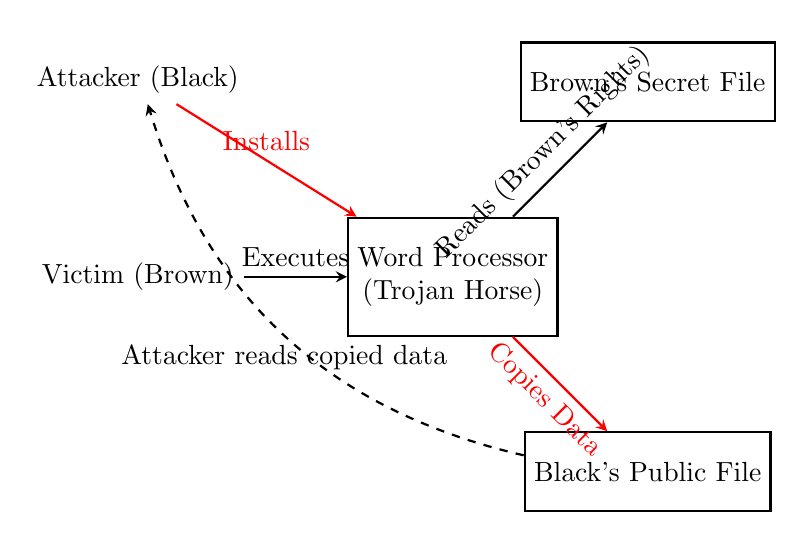
\begin{tikzpicture}[node distance=2.5cm, auto, thick, >=stealth]
        \node (attacker) {Attacker (Black)};
        \node[below of=attacker, node distance=2.5cm] (victim) {Victim (Brown)};
        \node[draw, rectangle, right of=victim, node distance=4cm, minimum height=1.5cm, align=center] (trojan) {Word Processor\\(Trojan Horse)};
        \node[draw, rectangle, above right of=trojan, node distance=3.5cm, minimum height=1cm] (secret) {Brown's Secret File};
        \node[draw, rectangle, below right of=trojan, node distance=3.5cm, minimum height=1cm] (shared) {Black's Public File};

        \draw[->, red] (attacker) -- node[above] {Installs} (trojan);
        \draw[->] (victim) -- node[above] {Executes} (trojan);
        \draw[->] (trojan) -- node[above, sloped] {Reads (Brown's Rights)} (secret);
        \draw[->, red] (trojan) -- node[below, sloped] {Copies Data} (shared);
        \draw[->, dashed, bend left] (shared) to node[below] {Attacker reads copied data} (attacker);
    \end{tikzpicture}
    \caption{The DAC Trojan Horse Problem. The Trojan inherits the victim's privileges to read a secret file, but abuses those privileges to copy the data into an object accessible to the attacker.}
    \label{fig:trojan_horse}
\end{figure}

In a Trojan Horse attack, a victim runs a malicious program. Because DAC grants the running process the same privileges as the victim, the process can legitimately read the victim's secret files. However, the program then maliciously writes that data into a different file owned by the attacker. DAC fails to stop this because the write operation is legitimately authorized under the victim's privileges.

\section{Mandatory Access Control (MAC)}
To solve the catastrophic data leakage inherent in DAC, high-security environments (such as military and intelligence agencies) employ \textbf{Mandatory Access Control (MAC)}. Under MAC, resource owners \textit{cannot} assign privileges. Instead, privileges are deterministically evaluated against system-wide policies defined by a security administrator. Popular MAC implementations include SELinux and AppArmor.

\subsection{Secrecy Levels and Labels}
MAC relies on the concept of \textit{clearance} for subjects and \textit{sensitivity} for objects. These classifications are composed of two parts:
\begin{enumerate}
    \item \textbf{A strictly ordered set of secrecy levels:} Hierarchical tiers of trust. For example, the US government utilizes: \texttt{Top Secret > Secret > FOUO > Unclassified}. NATO utilizes: \texttt{COSMIC Top Secret > NATO Secret > NATO Confidential > Unclassified}.
    \item \textbf{A set of non-hierarchical labels (compartments):} Subject-matter categories, such as \texttt{Nuclear, Crypto, Finance, Policy}.
\end{enumerate}

When combined, these elements form \textbf{Lattice-Based Access Control (LBAC)}. A classification is a pair $C = \{Level, Labels\}$. The relationships form a partial order (a mathematical lattice) defined by dominance:
\[ \{C_1, L_1\} \ge \{C_2, L_2\} \iff C_1 \ge C_2 \text{ and } L_2 \subseteq L_1 \]

A subject only dominates an object if the subject's hierarchical level is greater than or equal to the object's, \textit{and} the subject possesses all the specific compartment labels assigned to the object.

\subsection{The Bell-LaPadula Model (BLP)}
The most famous formalization of MAC for preserving confidentiality is the Bell-LaPadula (BLP) model. It overlays MAC rules on top of standard DAC. It relies on two fundamental MAC properties to prevent data leakage:
\begin{enumerate}
    \item \textbf{Rule 1 - The Simple Security Property (No Read Up):} A subject at a given secrecy level cannot read an object at a higher secrecy level.
    \item \textbf{Rule 2 - The Star Property ($\star$-property) (No Write Down):} A subject at a given secrecy level cannot write to an object at a lower secrecy level.
\end{enumerate}
Additionally, BLP defines \textbf{Rule 3 (Discretionary Security Property)}, requiring that any access must also be permitted by the underlying DAC access matrix.

The $\star$-property elegantly neutralizes the Trojan Horse problem. If a victim executes a Trojan, the process runs at the victim's high clearance level. The process can read the victim's high-secret files, but when the Trojan attempts to copy the data to the attacker's low-clearance file, the operation is rejected as an illegal ``write down.''

\subsubsection{Tranquility and Monotonic Flow}
The BLP model relies on the \textbf{Tranquility Property}, dictating that the security levels of active subjects and objects cannot change dynamically during execution. 

Because subjects can read down and write up, BLP creates a \textit{monotonic flow of information} toward higher secrecy levels. Data acts like a gas floating upwards; it can never organically descend to a lower classification. Consequently, BLP systems require highly \textit{trusted subjects}—special administrative processes exempt from the $\star$-property—to declassify or sanitize documents and move them down the lattice.

It is critical to note that BLP is designed exclusively for confidentiality. It \textit{does not address integrity} (preventing unauthorized modification of high-level data by low-level subjects). To secure integrity, systems often run a parallel model, such as the \textbf{Biba Model}, which limits modifications based on data trust levels.

\section{Conclusion}
Access control bridges the gap between verified authentication and safe resource utilization. Discretionary Access Control (DAC) provides the highly flexible, intuitive owner-centric model that dominates consumer and commercial software. However, due to its vulnerability to information leakage and Trojan attacks, strict environments layer Mandatory Access Control (MAC) atop DAC, utilizing mathematical models like Bell-LaPadula to forcefully dictate the flow of sensitive information.
